\chapter{Numerical Results}
\label{chap:numres}

In this chapter some application of the results described in
\cref{chap:flow,chap:analytsol} are presented. In
\cref{sec:hopsvsanalyt}, we begin by considering the bath energy for
an analytically solvable model and contrasting the analytical results
with the results obtained by hops.

\section{Some Remarks on the Methods}
\label{sec:meth}
The figures presented may feature error funnels whose origin is,
unless otherwise stated, estimated from the empirical standard
deviation of the calculated quantities due to the finite sample
size. As the quantities that are being calculated using HOPS are
essentially Monte Carlo integrals, those statistical errors scale as
\(1/\sqrt{N}\) with the sample size \(N\) and therefore controllable
besides being simple to estimate. Note however, that a certain number
of samples is required to estimate the standard deviation
correctly.

To tell whether some vector quantities\footnote{For example a time
  series.} \(X_1, X_2\) obtained with HOPS or otherwise are compatible
with each other or an analytical result, we consider the quantity
\(Δ=X_1 - X_2\). Assuming all numerical errors are negligible, we
demand that \(\abs{Δ} \leq σ_Δ\) for at least \(68\%\) of the entries
of the \(X_i\), where \(σ_Δ\) is the standard deviation due to the
stochastic sampling. This percentage is often displayed in legends as
a number in parentheses.

For the estimation of mean and standard deviation from trajectory
data, Welford's online algorithm is employed to avoid catastrophic
numerical cancellation~\cite{Welford1962Aug,Knuth1997}.

In all simulations discussed an Ohmic spectral density
\begin{equation}
  \label{eq:ohmic_sd}
  J(ω)=η ω \eu^{-\frac{ω}{ω_{c}}}\quad (ω>0)
\end{equation}
is used unless otherwise. This spectral density models an environment
with a physical energy spectrum that is bounded from below and allows
the application of the finite temperature method described
in~\cite{RichardDiss} \fixme{internal reference}. Also, \(J(0) = 0\)
ensures that there is a unique zero temperature state of the
bath. In~\cite{Kolar2012Aug} it is argued (under weak coupling
assumptions), that \(J(ω)\approx ω^γ\) with \(γ<1\) could lead to a
violation of the third law.  Physically, a scaling of the spectral
density \(\propto ω\) is connected to acoustic
phonons~\cite{Kolar2012Aug}.

In \cref{eq:ohmic_sd} \(η\) is a scaling
constant and \(ω_c\) (the cutoff frequency) regulates the decay of the
spectral density. The corresponding bath correlation function (BCF)
is
\begin{equation}
  \label{eq:ohmic_bcf}
  α(τ) = \frac{1}{π} ∫\dd{ω} J(ω) \eu^{-\iu ωτ} =
  \frac{η}{π}\qty(\frac{ω_c}{1+\iu ω_c τ})^2.
\end{equation}
We see that higher cutoff frequencies correspond to a faster decay of
the bath correlation function. This parameter provides control over
the ``Markovianity'' of the bath.

It may be remarked, that~\cref{eq:ohmic_bcf} does not correspond to a
simple sum of exponentials. As such it exercises the HOPS method and
serves as a model for a general bath correlation function. For use
with HOPS, a sum of exponentials must be fitted to the BCF. In
\cref{sec:hopsvsanalyt} we will see, that this is indeed a valid
strategy.

Throughout this chapter, we will only apply the nonlinear
method~\cite{Hartmann2017Dec} \fixme{rereference} (see also \cref{sec:nonlin_flow}).

\section{Comparison with an Analytical Solution}
\label{sec:hopsvsanalyt}
In \cref{chap:analytsol} and specifically \cref{sec:oneosc,sec:twoosc} an
analytical solution for a quantum Brownian motion like model was
derived. Using this solution, we are able to verify the results of
\cref{chap:flow} and benchmark the HOPS method. It will be shown, that
HOPS can indeed reproduce the \emph{exact} open system dynamics of the
bath energy flow.

\subsection{One Oscillator, One Bath}
\label{sec:oneosccomp}
For the simulations with HOPS the model \cref{eq:one_ho_hamiltonian}
was made dimensionless by choosing \(Ω=1\). Simulations were run for
both for zero temperature and a finite temperature with varying bath
correlation functions.

\begin{figure}[t]
  \centering
  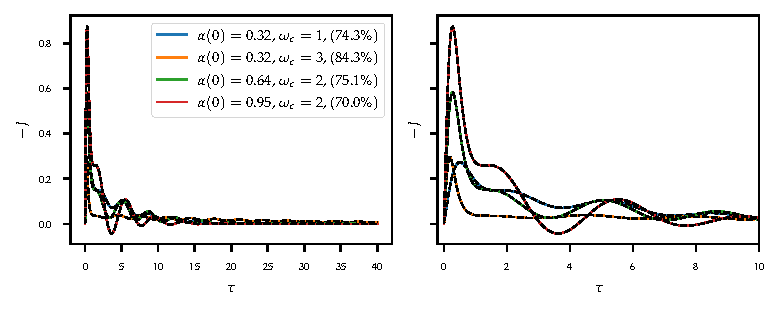
\includegraphics{figs/analytic_comp/flow_comp_zero.pdf}
  \caption{\label{fig:comp_zero_t} The bath energy flow \(-J\) for
    different parameters of the ohmic bath correlation
    function \cref{eq:ohmic_bcf}. The solid lines have been obtained
    with HOPS and the dashed lines using the analytic solution. A good
    agreement is evident visually and corroborated by the consistency
    values in the legend (see \cref{sec:meth} for an explanation).}
\end{figure}
\paragraph{Zero Temperature}
The bath energy flow \(J=∂_t\ev{H_\bath}\), from here on called simply
``the flow'' or ``bath energy flow'', for the zero temperature case
are illustrated in \cref{fig:comp_zero_t}. The results agree to a very
good accuracy, validating the findings of \cref{chap:flow}.

Although the simulations are primarily intended as a benchmark for
HOPS and a verification for the results of \cref{chap:flow} some
observations can be made in \cref{fig:comp_zero_t}. First, the flows
for different parameters all feature the characteristic spike
originating from the ``initial slip'', as explained in
\cref{sec:pure_deph} This is a quite universal feature and also shows
up on a single trajectory level suggesting that it is not strictly
related to an energy exchange with the bath but rather to the build-up
of interaction energy. This will be discussed further in
\cref{sec:prec}. \fixme{maybe a plot}The time dependence of the flow
also varies both with the shape of the BCF and the coupling
strength. For longer correlation times \(\propto 1/ω_c\) we find that
the flow initially decays much slower at the same coupling strength
(blue and orange lines) and exhibits stronger oscillations. After this
initial period the situation is reversed. For large coupling strengths
we can observe a ``backflow'' of energy out of the bath. In all cases
the flow features some oscillations and decays to zero which is
physical for the situation of a harmonic oscillator that gives all its
energy into a zero temperature bath.

The observed behaviour for longer bath memories may be qualitatively
understood by assuming that the system interacts with the same part of
the bath for a longer time and can therefore more efficiently transfer
energy. When the bath memory is short however, new interactions have
to be built up continuously which leads to a slower energy
transfer. Correspondingly, the system energy decays slower for shorter
bath memories \cref{fig:ho_zero_entropy}. Another explanation is a
resonance effect due to the peak of the BCF being located at \(ω_c\)
and the HO energy gap being one. We will discuss this point further in
\cref{sec:one_bath_cutoff} in the context of another model.

\begin{figure}[h]
  \centering
  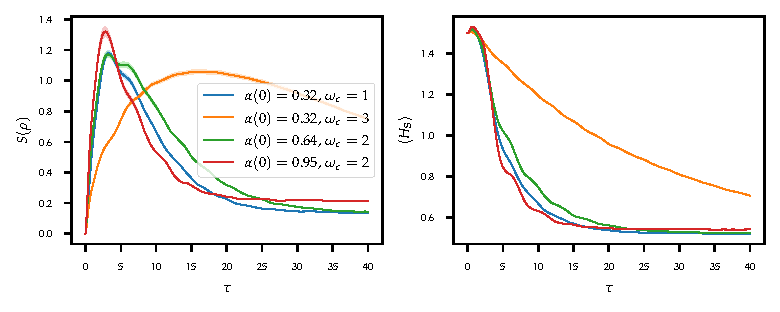
\includegraphics{figs/analytic_comp/entropy_zero.pdf}
  \caption{\label{fig:ho_zero_entropy} Left: The von Neumann entropy
    of the system state as a measure for entanglement with the
    bath. Right: The system energy as a function of time.}
\end{figure}
The ``backflow'' observed in \cref{fig:comp_zero_t} for stronger
coupling seems to diminish the advantage of stronger coupling over
larger bath memories. The decay of the red curve in
\cref{fig:ho_zero_entropy} is barely faster than the decay of the blue
curve, despite much larger coupling strength in the case of the red
curve. This may be due to the system interaction ``too long'' with a
given portion of the bath. Here we observe this behaviour for stronger
coupling which shortens the time-scale of energy exchange. It is an
interesting question for future work, whether we can also observe it
by further decreasing \(ω_c\).
\fixme{or now? if i have time}

Note however, that the steady state is not a product state as can be
seen by the residual entropy in \cref{fig:ho_zero_entropy} in the
cases where the steady state has been approximately reached. The
stronger the coupling, the larger the entanglement. The \(α(0)=0.95\)
simulation appears to be leading to a qualitatively different steady
state than the one with the same cutoff but weaker coupling
strength. This also manifests in a higher expected system energy in
the steady state.

The time dependence of the entropy the expectation value of the system
energy is markedly different for \(ω_c=3\). Although the coupling
strength is larger than in the \(α(0)=0.32,\, ω_c=1\) case the energy
loss of the system is markedly slower and the initial energy gain is
less pronounce. This is consistent with the flow in
\cref{fig:comp_zero_t}.

The simulation was run with a hierarchy depth of \(\norm{\vb{k}} \leq 5\)
(simplex truncation\footnote{see \cref{sec:hops_basics}}) and a BCF
fit with \(7\) terms taken from \cite{RichardDiss} which was also used
in the analytical solution. The harmonic oscillator Hilbert space was
truncated to \(15\) dimensions. As the initial state the first excited
state of the oscillator was chosen. Some \(N=5000\) trajectories have
been computed and lead to a quite satisfactory statistical error that
is small enough to be invisible in \cref{fig:comp_zero_t}. The
normalized standard deviation of the bath energy flow follows the
usual one-over-square-root rule as is illustrated in
\cref{fig:sqrt_conv}. Even after just \(N=1000\) trajectories the
normalized statistical error is on the order of \(10^{-3}\).
\begin{figure}[h]
  \centering
  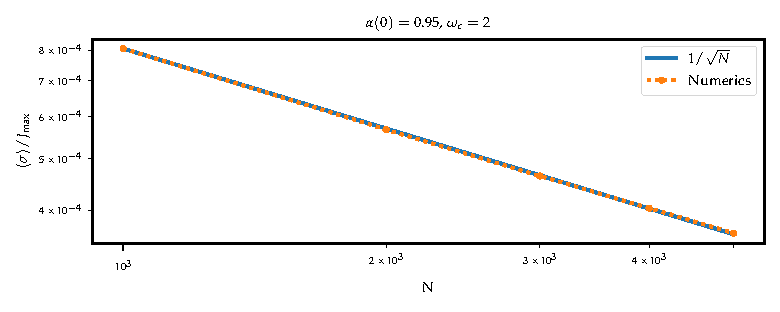
\includegraphics{figs/analytic_comp/sqrt_convergence.pdf}
  \caption{\label{fig:sqrt_conv} The (empirical) standard deviation
    (the statistical error) of the flow for the last configuration in
    \cref{fig:comp_zero_t} normalized by the maximum absolute value of
    \(J\).}
\end{figure}
\begin{figure}[h]
  \centering
  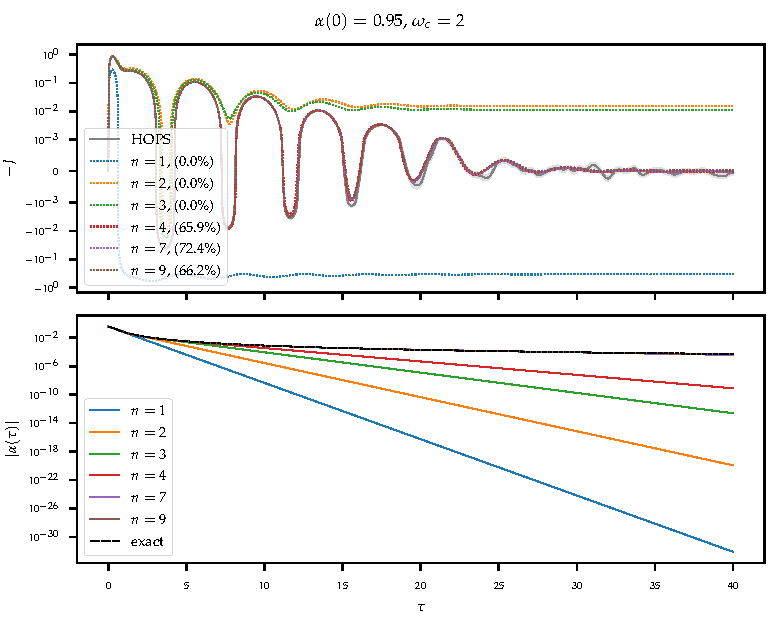
\includegraphics{figs/analytic_comp/analytical_terms_important.pdf}
  \caption{\label{fig:analytical_terms_important} Upper Panel: The analytical
    solution for the zero temperature bath energy flow using different
    numbers of terms in the BCF expansion in a symmetric logarithmic
    scale. For \(7\) terms the consistency (number in parentheses)
    with the numerical solution is best. Lower Panel: The absolute
    value of the approximated bath correlation function.}
\end{figure}
The analytical solution is quite sensitive to the quality of the BCF
expansion.  While one might expect that choosing the same number of
terms in the expansion for the analytical solution as was used for the
HOPS simulation, there still remains a systematic difference between
HOPS and the analytical solution, as the stochastic processes is
sampled using the full bath correlation function and more intricate
approximations~\cite{RichardDiss}.  Nevertheless, the best agreement
is found for using the same number expansion terms in both HOPS and
the analytical solution as is illustrated in
\cref{fig:analytical_terms_important}. Note that the consistency value
given in \cref{fig:analytical_terms_important} is different from the
one in \cref{fig:comp_zero_t}, as here a separate fit was made rather
than using the fit from \cite{RichardDiss}.

Interestingly, the solutions using a BCF expansion with three terms or
fewer lead to an unphysical non-zero steady state bath energy
flow. Considering specifically the case of one expansion this may be
related to the fact that now the BCF  term so that
\(α(τ)=G \exp(-Wτ)\) is related to a Lorentzian spectral density that
also includes unphysical negative frequencies.

\fixme{additional curve in plot, idea: start in the zero state ->
  product state is not the steady state, maybe longer times}

\paragraph{Finite Temperature}
\begin{figure}[t]
  \centering
  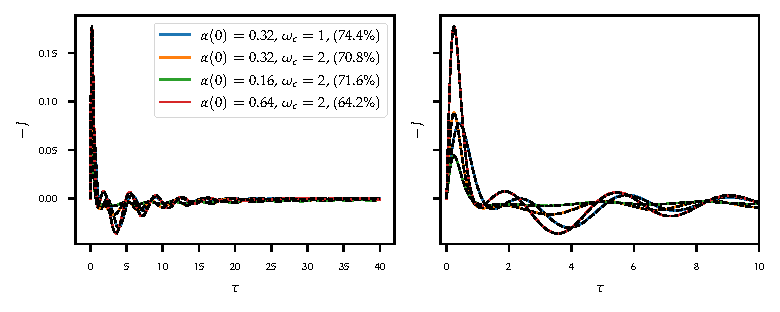
\includegraphics{figs/analytic_comp/flow_comp_nonzero.pdf}
  \caption{\label{fig:comp_finite_t} The bath energy flow \(-J\) of
    the quantum Brownian motion model for different parameters of the
    ohmic bath correlation function \cref{eq:ohmic_bcf} in the finite
    temperature \(T=1\) case. The presentation is equivalent to
    \cref{fig:comp_zero_t}.}
\end{figure}
The results for the finite temperature case are illustrated in
\cref{fig:comp_finite_t} for a temperature of \(T=1\). The setup was
otherwise equivalent to the zero temperature simulations, except for
the number of trajectories which was chosen to be \(N=10^5\).  Again
the high consistency values suggest that the findings of
\cref{chap:flow} are valid. The last case (\(α(0)=0.64,\, ω_c=2\)),
falls just short of the \(68\%\) mark, but agrees very well
visually. It is very probable, that simply more samples are required.

We find a similar behaviour to the zero temperature case, but this
time with a more pronounced flow out of the bath. For higher coupling
strengths, the flow amplitude is higher, as is also the case for lower
cutoffs.

One potentially contestable point in \cref{chap:flow} was the
appearance of the time derivative of the thermal stochastic process in
\cref{eq:pureagain}. The numerical method which is used to sample the
stochastic processes allows for a straight forward implementation of
this derivative so that no numerical derivatives are required and
there appears to be no problem.

As the dimensionality of the Monte Carlo integral underlying the
NMQSD/HOPS formalism is increased by the ``Stochastic Hamiltonian''
method, we observe markedly slower convergence as the variance of the
individual trajectories is higher.  In \label{fig:cons_dev_finite} the
convergence behaviour, as well the consistency with increasing
trajectory count are shown and this behaviour is observed. We also
find that in the more challenging regimes of stronger coupling or
longer bath correlation times the behaviour of the convergence is more
volatile, dipping into regions of inconsistency even at high sample
counts. While the mean difference between the numerical and the
analytical flow is always below the mean statistical error, larger
fluctuations can occur at certain points in time when a new region of
the probability space is sampled.

\begin{figure}[p]
  \centering
  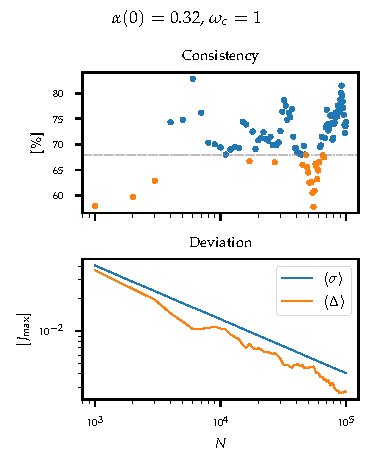
\includegraphics{figs/analytic_comp/consistency_development_0.pdf}
  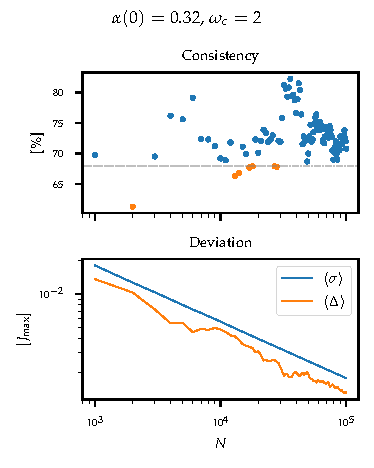
\includegraphics{figs/analytic_comp/consistency_development_1.pdf}
  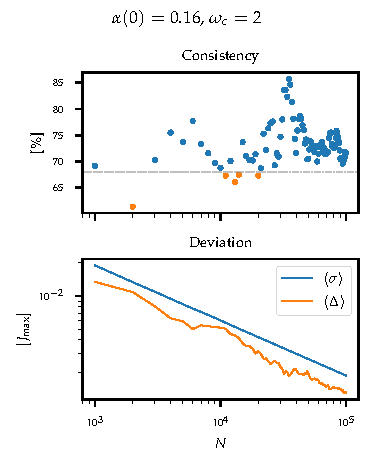
\includegraphics{figs/analytic_comp/consistency_development_2.pdf}
  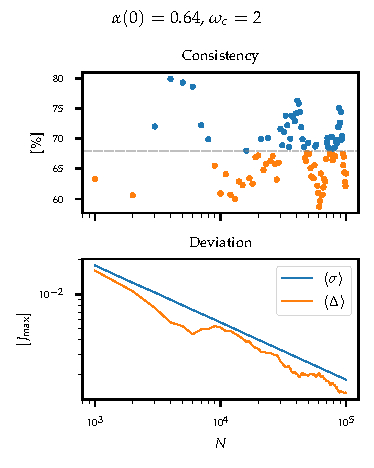
\includegraphics{figs/analytic_comp/consistency_development_3.pdf}
  \caption{\label{fig:cons_dev_finite} The convergence of the flows of
    \cref{fig:comp_finite_t} with increasing trajectory count. The upper
    panels show the consistency, where the grey marks the \(68\%\)
    threshold for consistency. The lower panel shows the time averaged
    values of the statistical error \(\ev{σ}\) and the deviation from
    the analytical result \(\ev{Δ}\) by the maximum absolute value of
    \(J\).}
\end{figure}

% The advantage of the ``Stochastic Hamiltonian'' method for finite
% temperature (see \cref{eq:thermalh}) is that one doesn't have to deal
% with the finite temperature BCF that does decay markedly slower than
% its zero temperature counterpart as is illustrated in
% \cref{fig:bcf_decay}. Generically, more terms in the BCF expansion
% would be required to capture the algebraic decay appropriately.

% \begin{figure}[t]
%   \centering
%   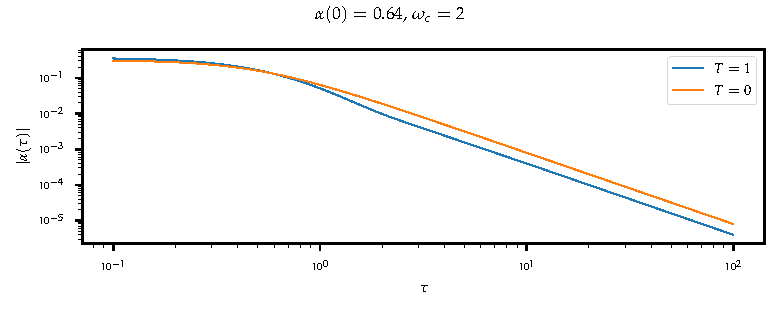
\includegraphics{figs/analytic_comp/bcf_decay.pdf}
%   \caption{\label{fig:bcf_decay} The absolute value of the Ohmic BCF
%     used in the last simulation of \cref{fig:comp_zero_t}.}
% \end{figure}

\subsection{Two Oscillators, Two Baths}
\label{sec:twoosccomp}

The model of \cref{sec:oneosc} was generalized to two oscillators
coupled to two separate baths in \cref{sec:twoosc} and
\cref{eq:hamiltonian_two_bath}. In this section we simulate this model
and compare the results with the analytical solution.

For simplicity, the parameters were chosen symmetric so that the
frequencies of both oscillators are the same \(Ω=Λ=1\). As before,
\(Ω\) defines the energy unit. The zero temperature bath correlation
functions of both baths were chosen identically with a cutoff
frequency \(ω_c=2\). The intra-oscillator coupling was chosen as
\(γ=0.5\). The hierarchy was truncated so that \(\abs{\vb{k}}\leq 3\) and a BCF
expansion with five terms was chosen to limit memory demands.
\fixme{mention number of samples}

To limit the variance the temperature of one of the baths was set to
zero, so that only one thermal stochastic process was introduced. The
other bath was chosen to have \(T=0.6\). The ground state of the
system Hamiltonian \(\ket{0}\otimes \ket{0}\) was chosen as the
initial state of the oscillators.

The main challenge of simulating the model \cref{eq:hamiltonian_two_bath} is
the dimension of the system Hilbert space which is constrained by the
available memory. In the simulation discussed here, each oscillator
was truncated at \(9\) levels leading to \(9^2 = 81\) dimensions in
total\footnote{This is a naive method of truncation, but sufficient
  for the purposes of this work.}. The effect of a too drastic
truncation of the system Hilbert space can be seen in
\cref{fig:insufficient_levels}. At the temperature chosen the mean
level occupation of a harmonic oscillator is given by the Bose distribution
\begin{equation}
  \label{eq:harm_mean_occ}
  \ev{n} = \frac{1}{\eu^{Ωβ}-1} \approx 0.23 < 1.
\end{equation}
Nevertheless, quite more than two levels are required per
oscillator. This may be due to a required minimal resolution of the
position operators that occur in the model
\cref{eq:hamiltonian_two_bath} which is formulated with position space
in mind.

The final result can be studied in \cref{fig:sufficient_levels}. We
find good, but not excellent agreement. Based on the results of
\cref{sec:oneosccomp} however, it can be argued that this result is
sufficient to corroborate the validity of the results of
\cref{sec:multibath}. With more computational effort\footnote{Mainly
  more BCF expansion terms.} and fine-tuning of parameters an even
better agreement between the analytical and the numerical results may
be achieved.
\begin{figure}[h]
  \centering
  \begin{subfigure}[t]{.49\linewidth}
    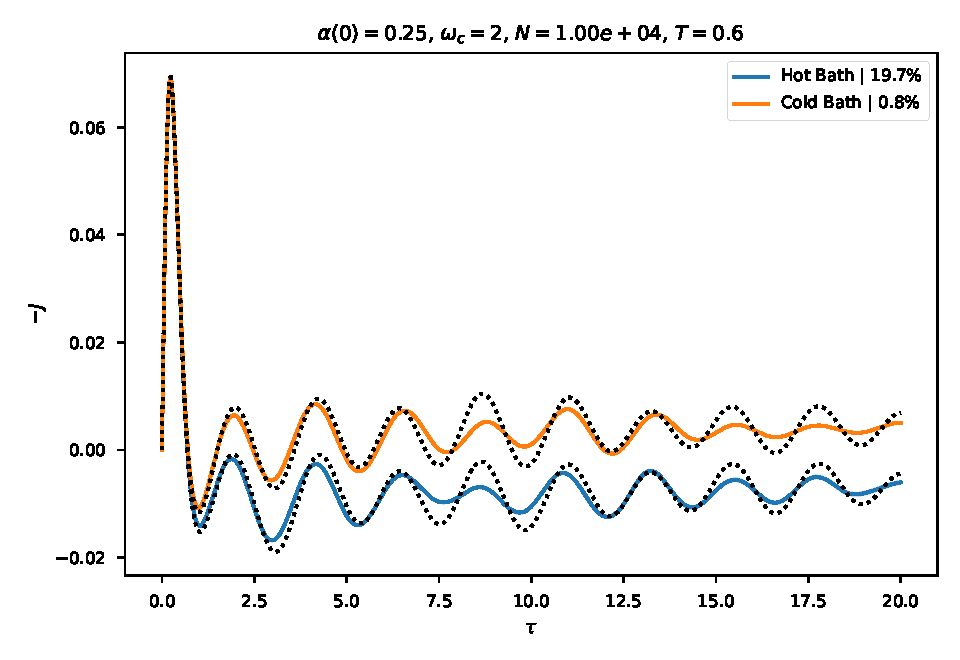
\includegraphics{figs/analytic_comp/comparison_two_5bcf_5ho.pdf}
    \caption{\label{fig:insufficient_levels}\(\dim\hilb_\sys=25\).}
  \end{subfigure}
  \begin{subfigure}[t]{.49\linewidth}
    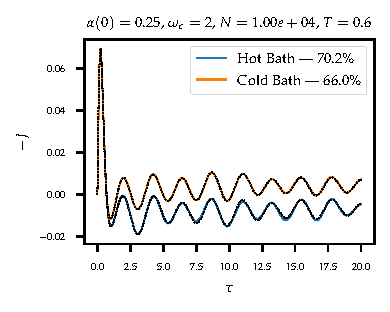
\includegraphics{figs/analytic_comp/comparison_two_ho.pdf}
    \caption{\label{fig:sufficient_levels}\(\dim\hilb_\sys=81\).}
  \end{subfigure}
  \caption{\label{fig:comp_two_bath} The bath energy flows for
    the model \cref{eq:hamiltonian_two_bath}, where the dashed lines
    correspond to the analytical solutions.}
\end{figure}

\Cref{fig:comp_two_bath} exhibits some interesting features. The
initial slip peak in the bath energy flows is identical for both baths
and independent of temperature as suggested by the discussion in
\cref{sec:pure_deph}. As is expected, the hot bath looses energy and
the cold bath gains energy, while this process is modulated by the
intra-oscillator coupling. It follows from the analytical solution
that eventually a steady state without oscillations will be reached.

Interestingly, the zero temperature bath flow converges very much
faster than the finite temperature flow despite the whole system being
connected, at least indirectly, to the hot bath. The reason for this
is that the derivative of the thermal stochastic process \(\dot{ξ}\)
dominates the variance of the flow for each trajectory. This is also
the reason that expressions depending on the hierarchy states rather
than time derivatives of stochastic processes are preferred as
discussed in \cref{sec:general_obs}.

\fixme{show simulation with insufficient HO levels} We have shown that
the findings of \cref{chap:flow} are consistent with
\cref{chap:analytsol} and that through a careful choice of the HOPS
parameters such as hierarchy depth, Hilbert space dimension and BCF
expansion the exact open system dynamics of the bath energy flow can
be reproduced. The statistical error can be made arbitrarily small by
increasing the trajectory count. For a given target error, the
trajectory count can be estimated by the empirical standard deviation
of a given observable.

For future work there remains the generalization of the work in this
section and \cref{chap:analytsol} to time dependent couplings and
Hamiltonians. Because the NMQSD and also HOPS are largely agnostic of
these factors, we may safely assume that the results of the comparison
will be similar to the ones presented here.

\section{Precision Simulations for a System without Analytical
  Solution}
\label{sec:prec_sim}
In this section, we will study the energy flow of a simple model
connected to zero temperature bath. Both the characteristics of the
flow mediated by the concrete form of the bath correlation function
and the performance of the HOPS method itself will be investigated. We
will find that the numerics do indeed yield very consistent results
and that the specifics of the energy flow depend very much on the
spectral density.

An analytical solution to a given open system is generally not known,
so that another indicator of the proper choice of HOPS parameters may
be required. In this section we will briefly demonstrate some high
precision simulations of a single qubit coupled to a single zero
temperature bath. The corresponding Hamiltonian is
\begin{equation}
  \label{eq:one_qubit_model}
  H = \frac{1}{2} σ_z + \frac{1}{2} ∑_λ\qty(g_λ σ_x^† a_λ + g_λ^\ast
  σ_x a_λ^†) + ∑_λ ω_λ a_λ^\dag a_λ,
\end{equation}
where we've chosen \(H\) to be dimensionless\footnote{The energy scale
is set by the system Hamiltonian.}.

In the language of HOPS this corresponds to \(H_\sys=σ_z/2\),
\(L=σ_x/2\). We again choose the Ohmic BCF as explained in
\cref{sec:meth}. Throughout this section we choose the ``up'' state
\(H_S\ket{1} = 1/2\ket{1}\) as the initial state of the system.

The main measure of convergence for variables other than the
trajectory count are consistency conditions. The simplest one
available to us is energy conservation which allows us to calculate
the expectation value of the interaction energy through integration of
the bath energy flow. The interaction energy obtained in this way can
then be compared to the interaction energy obtained directly as shown
in \cref{sec:intener}.  For time dependent Hamiltonians, the power
must be considered similarly.

To check for converge we generally set all parameters to a value which
may be safely above the required optimum and vary one parameter. This
is a procedure that could be automated in future work. The main
sources of systematic deviations for the model
\cref{eq:one_qubit_model} are the quality of the sampling of the
stochastic process and the cutoff of the hierarchy. The first becomes
important when the cutoff frequency is large and the BCF vanishes
rapidly and has to be resolved on shorter time scales. The second is
important when the cutoff frequency is smaller and the bath has a
longer memory.

\subsection{Stochastic Process}
\label{sec:stocproc}
For studying the convergence behaviour regarding the sampling of the
stochastic process we chose the cutoff as \(\norm{\vb{k}} \leq 4\)
(simplex truncation\footnote{see \cref{sec:hops_basics}}),
\(N=4.5 \cdot 10^5\) trajectories and an Ohmic BCF with \(α(0)=1.6\)
and \(ω_c=4\). The high cutoff was chosen to provide the most
challenging setting for the sampling. The sampling method uses the
``Fast Fourier Transform'' (FFT) as described
in~\cite{RichardDiss}. As the system Hilbert space dimension is small,
a BCF expansion with seven terms was employed.

The main parameter of this method is the accuracy of the FFT. The
implementation compares the BCF and its FFT approximation on the time
interval of the simulation and chooses the internal
parameters\footnote{The number of time grid points and the integral
  boundaries in frequency space.} so that the difference normalized by
\(α(0)\) is smaller than a given value \(ς\).

\begin{figure}[h]
  \centering
  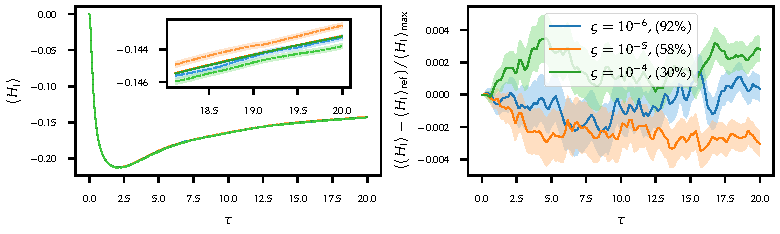
\includegraphics{figs/one_bath_syst/stocproc_systematics_interaction}
  \caption{\label{fig:stocproc_systematics} Left panel: The
    interaction energy of the model \cref{eq:one_qubit_model} for
    \(α(0)=1.6\) and \(ω_c=4\) using different precisions for the
    sampling of the stochastic process. The dashed lines are obtained
    using energy conservation while the solid lines are obtained
    directly as in \cref{sec:intener}. The consistency between the too
    is given in the legend of the right panel. Right panel: The
    difference of the interaction energies obtained using energy
    conservation and directly. The values are normalized by the
    maximal absolute value of the interaction energy.}
\end{figure}
\Cref{fig:stocproc_systematics} illustrates the effect of this
parameter. We find very good qualitative agreement for all values of
\(ς\). The indirectly calculated value of then interaction energy
shows some fluctuation between the settings, but the value calculated
directly is very stable as can bee seen in the inset of
\Cref{fig:stocproc_systematics}.

\begin{wrapfigure}[15]{o}{0.5\textwidth}
  \centering
  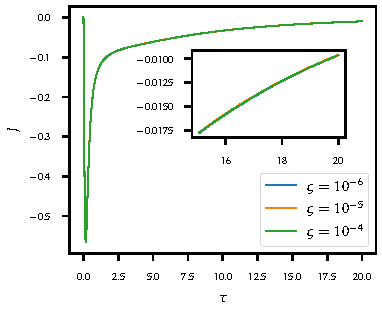
\includegraphics{figs/one_bath_syst/stocproc_systematics_flow}
  \caption{\label{fig:stocprocflow}The bath energy flow of the model
    \cref{eq:one_qubit_model} for \(α(0)=1.6\) and \(ω_c=4\) using
    different precisions \(\varsigma\) for the sampling of the
    stochastic process.}
\end{wrapfigure}
The same behaviour can be observed with the bath energy flow in
\cref{fig:stocprocflow}, which demonstrates near-identical results.

Only in the \(\varsigma=10^{-6}\) case however, compatibility is
satisfied at the given sample count. This is due to the fact that here
multiple values that are obtained in different ways, namely system
energy and the flow, have to be considered. The system energy depends
on the zeroth hierarchy order only whereas the flow additionally
depends on the first hierarchy states and has to be numerically
integrated.

The development of the consistency of trajectory count \(N\) can be
studied in \cref{fig:stocproc_consistency_dev}. Only for the highest
precision case we have a consistent picture. For lower precision, the
consistency fluctuates and only occasionally surpasses \(68\%\). For
the lower precisions we find that they initially demonstrate
compatibility (until about \(N=10^4\)) but eventually diverge from the
exact\footnote{The result that demonstrates compatibility
  consistently.} result. It is therefore important to consider the
dependence of the compatibility on the sample count \(N\) to judge the
veracity of the simulation results.
\begin{figure}[p]
  \centering
  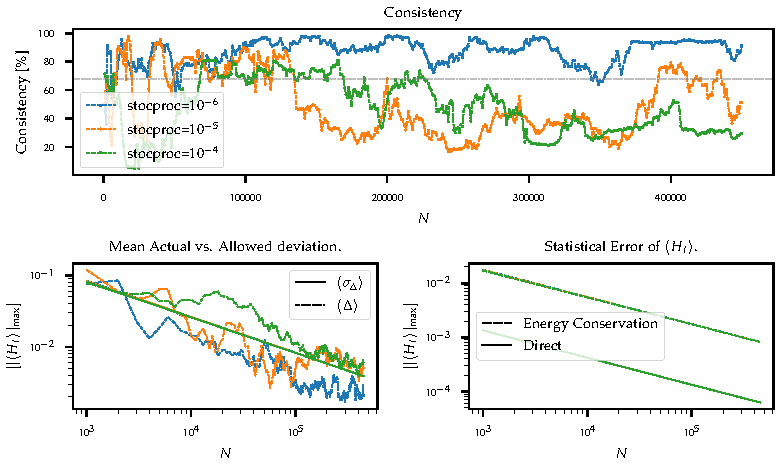
\includegraphics{figs/one_bath_syst/stocproc_systematics_consistency}
  \caption{\label{fig:stocproc_consistency_dev} Upper panel: The
    compatibility of the flow (direct computation vs. energy
    conservation) of the model \cref{eq:one_qubit_model} for
    \(α(0)=1.6\) and \(ω_c=4\) using different precisions
    \(\varsigma\) for the sampling of the stochastic process in
    relation to the trajectory count \(N\). Lower left: The time
    averaged difference (dashed) and the time averaged standard
    deviation of the difference (solid) as a function of trajectory
    count. Only for the smallest \(\varsigma\) the difference is
    consistently smaller than the standard deviation of the
    difference. Lower right: The time averaged statistical errors of the interaction
    energy calculated directly (solid lines) and indirectly through
    energy conservation (dashed lines).}
\end{figure}

Apart from being closer to the correct result, the direct computation
of the interaction energy has the advantage of providing faster
convergence\footnote{See \cref{fig:stocproc_consistency_dev}, lower right
  panel.}.

\subsection{Hierarchy Truncation}
\label{sec:trunc}
As the effect truncation depth has already been studied thoroughly
in~\cite{RichardDiss}, we will keep the discussion short.  We chose
\(N=4.5 \cdot 10^5\) trajectories and an Ohmic BCF with \(α(0)=0.8\)
and \(ω_c=2\). Again, seven a BCF expansion with seven terms have been
used. The coupling strength has been chosen with the help of
\cref{sec:pure_deph}, so that the interaction energy is of a similar
order of magnitude as in the discussion
above. \Cref{fig:k_systematics} shows that there seems to be no
improvement in accuracy or even change in the value of the flow for
\(\norm{\vb{k}}\geq 4\). However, the inset in the left panel
demonstrates that the direct result differs slightly for
\(\norm{\vb{k}} = 2\), which demonstrates that an adequate choice of
truncation depth is important.
\begin{figure}[h]
  \centering
  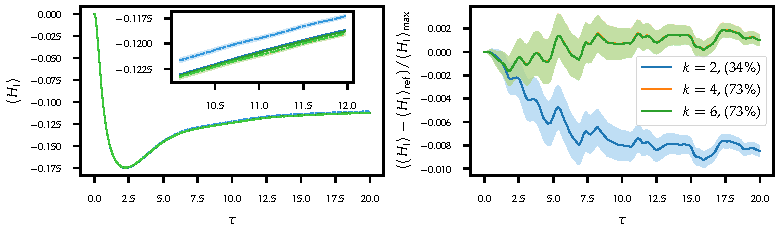
\includegraphics{figs/one_bath_syst/k_systematics_interaction}
  \caption{\label{fig:k_systematics} The same as
    \cref{fig:stocproc_systematics} but for \(α(0)=0.8\) and
    \(ω_c=2\) and for various truncation depths \(k=\norm{\vb{k}}_{\mathrm{max}}\).}
\end{figure}

The observed behaviour may be due to the fact that only zeroth and
first hierarchy depth states contribute to the result. For a
truncation depth of four, the first hierarchy state does not ``see''
the truncation any more. The deviation of the system energy from the
highest precision value is shown in
\cref{fig:k_systematics_system}. We see that the normalized difference
of the \(\norm{\vb{k}} = 2\) case from the \(\norm{\vb{k}} = 6\) is on
the same order of magnitude for system energy and interaction energy
which contradicts the aforementioned explanation. Also, the results
\(\norm{\vb{k}} = 4,6\) agree perfectly for both energies.
\begin{figure}[h]
  \centering
  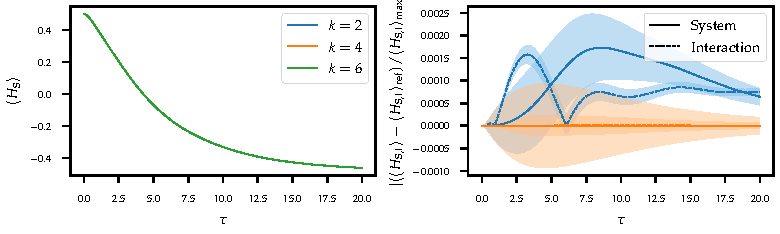
\includegraphics{figs/one_bath_syst/k_systematics_system}
  \caption{\label{fig:k_systematics_system} Left panel: The system
    energy of the model \cref{eq:one_qubit_model} with \(α(0)=0.8\)
    and \(ω_c=2\) and for various truncation depths
    \(k=\norm{\vb{k}}_{\mathrm{max}}\). Right panel: The difference between
    the \(k=4\) result and the results with \(k<4\) normalized by the
    maximal absolute system energy (solid lines) and the same for the
    interaction energy (dashed lines).}
\end{figure}

\begin{wrapfigure}[12]{o}{0.3\textwidth}
  \centering
  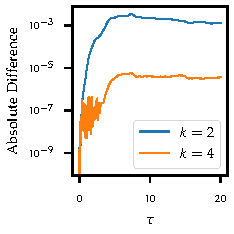
\includegraphics{figs/one_bath_syst/trajectories_not_same}
  \caption{\label{fig:notsame} The norm of the difference of a
    normalized single trajectory to the \(\norm{\vb{k}} = 6\) case.}
\end{wrapfigure}
\Cref{fig:notsame} demonstrates, that there is still a difference
greater than the machine epsilon on the level the trajectories. This
difference however, is small enough not to impact observables.

Summarizing, it may be said that the HOPS parameters have to be chosen
carefully for precision simulations, but that lower precision results
already give a \emph{very} good qualitative picture.

\fixme{maybe describe integration and error propagatation and time distribution.}
\fixme{maybe run a simulation with more hierarchy depth and more bcf
  terms, check whether there is a mistake}
It remains for future work to perform precision studies the
systematics of the finite temperature flow and modulated
Hamiltonians. In the following sections we will look at some examples
of physically interesting systems with less focus on the systematics
of convergence.

\subsection{Dependence on the Cutoff Frequency}
\label{sec:one_bath_cutoff}
We now consider precision simulations of the spin-boson like system
with varying cutoff frequency. To make the interaction energies
comparable to each other, the BCF normalization of section
\cref{sec:pure_deph} is being used. Because of the small size of the
Hilbert space, we were able to choose a HOPS
configuration\footnote{\(\norm{\vb{k}}\leq 7\), seven BCF terms,
  \(\varsigma = 10^{-6}\)} that yields high-accuracy results, based on
the results of the previous section. A detailed account of the
consistency is given in \cref{fig:omega_interaction_consistency}. The
only problematic result is the one for \(ω_c=1\), but there is good
qualitative consistency in this case. For all simulations
\(N=5\cdot 10^{5}\) trajectories were computed. The results of these
simulations are summarized in \cref{fig:omega_systematics_system}.
\begin{figure}[h]
  \centering
  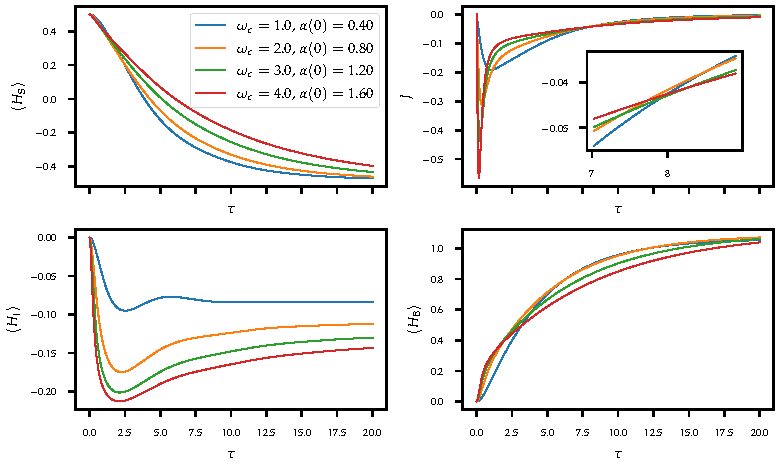
\includegraphics{figs/one_bath_syst/omega_energy_overview}
  \caption{\label{fig:omega_systematics_system} Energy overview for the
    model \cref{eq:one_qubit_model} for various coupling strengths and
     cutoff frequencies. The curves are converged out, and the error
    funnels are not visible.}
\end{figure}

Let us preface the following discussion with a note of caution. All
the discussed phenomena are specific to the minimal model
\cref{eq:one_qubit_model}, although sometimes similarities to
phenomena observed in \cref{sec:hopsvsanalyt} can be seen. Whether
there is some universality to the results obtained is an interesting
question for a more detailed future detailed study.\fixme{Remove this?}

The interactions energy expectation values, despite being in the same
order of magnitude, differ significantly. This illustrates the
limitation of the estimate in \cref{sec:pure_deph}. Better estimates
of the interaction energy and thus interaction strength may be derived
from ideas similar to the ones discussed in
\cref{sec:normest}. Besides the magnitude, the qualitative time
dependence of the interaction energies varies, especially between the
\(ω_c=1\) configuration and the others.

The blue (\(ω_c=1\)) curve exhibits two pronounced turning points as
opposed to one as the others do. This behaviour may be interpreted as
non Markovian. Further, despite having the weakest overall coupling
strength \(α(0)=0.4\) the system energy falls off the fastest after a
short period where it is above the other configurations. This
behaviour is also visible in the bath energy expectation value, where
the blue almost reaches the same levels as the \(ω_c=2\) configuration
for \(τ\gtrsim 5\).

The flow is generally negative (the bath gains energy) and decays
after an initial peak. All the flow graphs appear to be crossing in
about the same point \(τ\approx 7.7\) after which their ordering by
magnitude is reversed.  The inset shows that the crossing is not
precisely at the same point, nevertheless further investigation of
this phenomenon may of interest in the future. The decay is
faster for higher cutoff frequencies and stronger couplings. Despite
the higher interaction energies and coupling strengths, the
high-cuttoff simulations exhibit a slower energy transfer after the
initial peak as decayed sufficiently, with the system energy falling
slower and the bath energy rising slower. The situation is generally
reversed for short times \(τ\lesssim 2.5\), because here the build-up
of interaction energy is significant. Despite the moving peaks in the
flow, the location of the first extremum in is remarkably stable.

The presentation in \cref{fig:omega_systematics_system} is not
conducive to comparing the actual performance of the energy transfer,
because of the variable shape of the spectral density and the chosen
normalization. Because the maximum of the Ohmic spectral density is
located at \(ω_c\) the special observed energy transfer behaviour for
\(ω_c=1\) is likely due to a resonance effect as the system energy
level spacing is unity.

The dissipator of the master equation for this two level system only
depends on the value of the spectral density at the level
spacing~\cite[p. 66]{Rivas2012}\footnote{There \(L=σ_{+}\), but this
  has no bearing on the connection to \(ω_{0}\).}  (\(ω_{0}=1\) here),
so that it is reasonable to expect, that there may be variations
whenever its magnitude at this point changes.  On the other hand, a
strong dependence of the flow on the shape of the bath correlation
function beyond lamb-shift like influences, as we will find below, is
a token of the departure from the Markovian and weak coupling
regime\fixme{Here, some master equation comparison would be nice.}.

\paragraph{Energy Transfer Characteristics}
For a systematic study of resonance, we first compare the flow for
shifted ohmic spectral densities\footnote{See \cref{sec:shift_sp} for
  details.} with the same scaling and cutoff frequency \(ω_c=2\). We
turn off the interaction smoothly\footnote{A smoothstep function of
  order two with a transition period of two. See
  \cref{sec:smoothstep}.} over two time units before the system has
reached its steady state and compare how much energy has been
transferred in terms of the final bath and system energies and the
loss due to the modulated coupling.

\begin{wrapfigure}[12]{O}{0.3\textwidth}
  \centering
  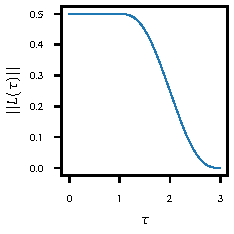
\includegraphics{figs/one_bath_syst/L_mod}
  \caption{\label{fig:L_mod} The smooth modulation of the coupling
    operator \(L(τ)\).}
\end{wrapfigure}
The less energy the system has at the end of the process and
the more the bath has taken up, the better the performance of
transfer. If the interaction energies are on the same scale, the
decoupling costs should be roughly the same. Otherwise, they may heat
to an additional modulation of system and bath energies between the
different simulations.

To make space for the shifted bath correlation functions, the system
energy gap has been set to four so that \(α(0)=8\) represents a quite
reasonable coupling strength.

The results for three shifts are presented in
\cref{fig:resonance_analysis}. For all shifts the spectral density has
a finite value at the system energy spacing, but in the \(ω_s=2\)
case, the resonance condition is fulfilled. Indeed, the energy
transfer out of the system is the best for the resonant case (see
\cref{fig:resonance_analysis}, middle panel). The change in total
energy due to the decoupling of the bath is moderately higher than in
the resonant case than in the \(ω_s=1\) case, but the final system
energy is the lowest. \fixme{The decoupling seems to affect mainly the bath
energy (see left panel). Should I say so?}
\begin{figure}[ht]
  \centering
  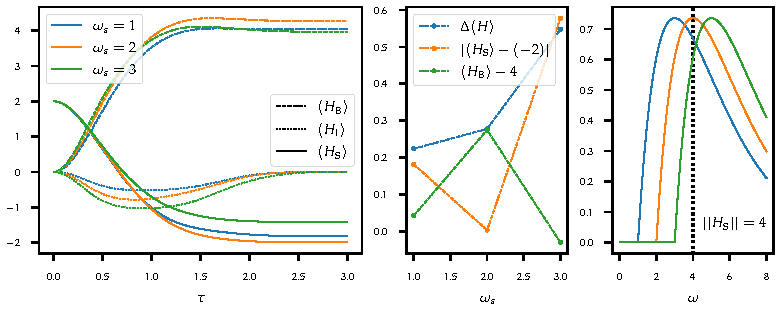
\includegraphics{figs/one_bath_syst/resonance_analysis}
  \caption{\label{fig:resonance_analysis} Left
    panel: The system, bath and interaction energies for various Ohmic
    BFCs with \(α(0)=8,\,ω_c=2\) shifted by \(ω_s\). Mid panel: The
    difference in total energy, the distance of the system energy to
    the ground state energy and the distance of the bath energy to the
    initial system energy. Right panel: The spectral density for the
    three shift values. \(\norm{H_\sys}\) does mean in this case, that
    the energy level spacing of the system is \(4\).}
\end{figure}\fixme{nicer}

The third simulation with \(ω_s=3\) exhibits the worst performance
with the lowest final bath energy the highest residual system energy
and the highest change in total energy due to high interaction
energy.\fixme{does this have anything to do with the lamb-shift?}

Were the interaction turned off abruptly, the system and bath energies
would remain untouched. Turning the interaction off in finite time
reduces the energy introduced into the system in the cases discussed
here. System and bath energy must therefore compensate part of the
negative interaction energy after the system is decoupled from the
bath. Hence, the generic lowering of system and bath energy after
decoupling.

% Turning of the interaction leads mostly to a reduction of the final
% bath energy (see the middle panel).  This effect will also appear in
% most of the cases discussed below. When deriving a master equation for
% this two level system~\cite[p. 68]{Rivas2012}, there occurs a lamb
% shift term that acts as a correction to the unitary evolution of the
% system. Turning the interaction off adiabatically removes this leads
% to a change in what one may define as system energy in this case. In
% the case discussed here, the coupling is not weak so that this
% explanation may only serve as a means of analogy. Compensating for the
% negative interaction energy, the system and bath energy expectation
% value both fall when the coupling is turned off.\fixme{is this
%   reasonable?}

% For an ohmic spectral density the lamb shift energy is
% \begin{equation}
%   \label{eq:lshift_twolevel}
%   2Δ=\eu^{-1/ω_{c}}\,\mathrm{Ei}\qty(\frac{1}{ω_{c}}) - ω_{c},
% \end{equation}
% which is negative for all the cases discussed here and may account for
% some part of the negative interaction energy. In this way, the removal
% of the bath would


Generally the maximal absolute interaction energy is roughly
proportional to the shift\fixme{maybe due to the fact that only higher
  frequency modes are available}, so that the short term interaction
strength as measured by the interaction energy expectation value is
not only dependent on the width and total norm of the spectral
density, but also on its absolute distribution in frequency space. The
worse performance of the large shift case may be due to the lack of
coupling to low frequency modes\fixme{this is speculation, should I
  remove it?} or the greater asymmetry of the spectral density around
the resonance frequency.

Due to the asymmetry of the spectral density, the simulations for
\(ω_s=1\) and \(ω_s=3\) are not directly comparable. A repetition of
this investigation with a (pseudo~\cite{Mukherjee2020Jan}) Lorentzian
spectral density and for different interaction
time-frames\footnote{steady state vs. transient states} is left for
future work.

The longer term picture is being studied in
\cref{fig:resonance_analysis_steady}. We see broadly similar energy
transfer characteristics for \(ω_{s}=1\) and \(ω_{s}=2\), where the
off-resonant may be marginally advantageous. The left panel shows,
that although the system energy is lower in the resonant case, the
situation is reversed during the decoupling. However these effects are
quite marginal and should be taken with care. The system energy
difference amounts to
\(\Delta\langle H_\mathrm{S}\rangle=0.00397\pm 0.00010\), but only the
statistical error has been taken into account. The simulations were
run with \(N=10^{4}\) samples and the same HOPS settings as in the
discussion above, so that some confidence may be placed in them. For
\(ω_{s}=3\) the steady state has not been reached yet and the energy
transfer is incomplete. In comparison with
\cref{fig:resonance_analysis} the system energy is generally lower but
the disturbance of system and bath energy due to the decoupling is
greater but to the advantage of the final system energy.
\begin{figure}[h]
  \centering
  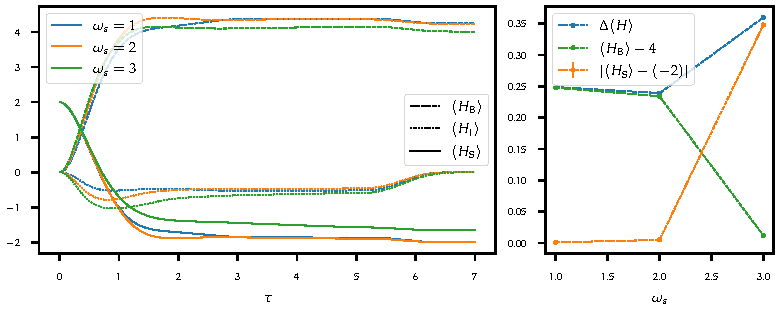
\includegraphics{figs/one_bath_syst/resonance_analysis_steady}
  \caption{\label{fig:resonance_analysis_steady} The same as
    \cref{fig:resonance_analysis} but for a longer coupling time.}
\end{figure}

To study the effect of the bath memory, we use Ohmic spectral
densities with varying \(ω_c\) that have been shifted and scaled so
that their peaks coincide and the resulting interaction energies are
comparable.

The results that can be obtained are very much dependent on the
timing. \Cref{fig:markov_analysis} has been arrived at by tweaking the
time point of decoupling so that an extremum in the \(ω_{c}=1\) curve
is captured. This leads to an advantageous transfer performance with a
lower system energy and a higher bath energy and similar cost in terms
of total energy change.
\begin{figure}[h]
  \centering
  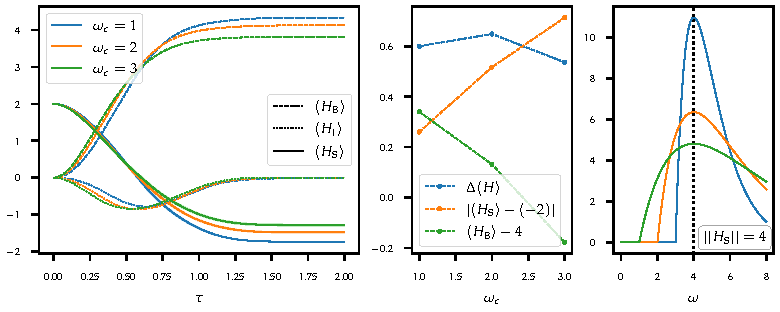
\includegraphics{figs/one_bath_syst/markov_analysis}
  \caption{\label{fig:markov_analysis} The same as
    \cref{fig:resonance_analysis} but for shifted spectral densities
    various cutoff frequencies.}
\end{figure}

For slightly longer coupling times, we find in
the exact opposite picture as can be ascertained from \Cref{fig:markov_analysis_longer}.
\begin{figure}[h]
  \centering
  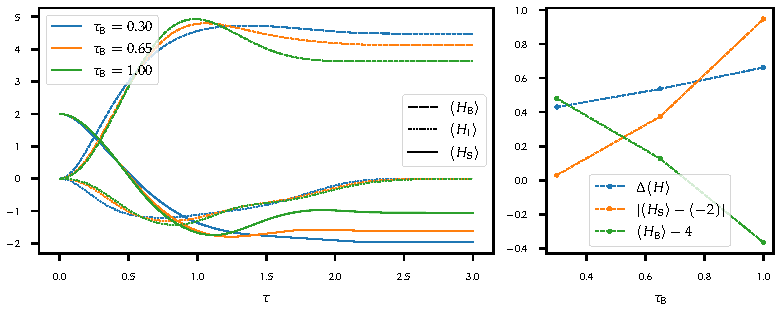
\includegraphics{figs/one_bath_syst/markov_analysis_longer}
  \caption{\label{fig:markov_analysis_longer} The same as
    \cref{fig:markov_analysis} but with slightly different timing.}
\end{figure}
The increased bath memory time allows for ``back flow'' of energy and
so the performance of energy transfer is strongly dependent on the
precision of control.\fixme{Should i be more exacting with regards
  to mentioning sample counts etc?}

For even longer times we find in \cref{fig:markov_analysis_steady},
that the advantage of longer bath memory vanishes. But here the
situation is complicated by the fact, that the steady state for the
\(ω_{c}=1\) case has not been reached.\fixme{Revise this after running
the simulation.}
\begin{figure}[h]
  \centering
  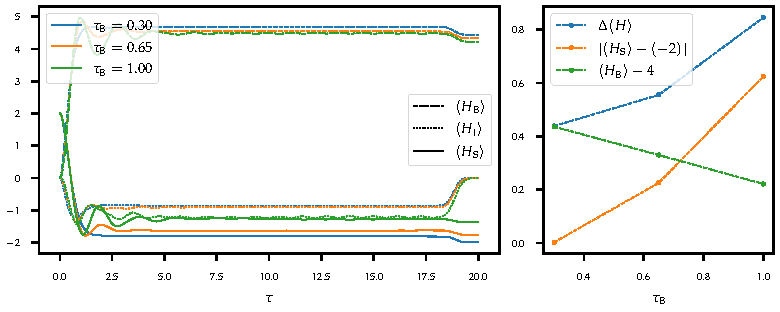
\includegraphics{figs/one_bath_syst/markov_analysis_steady}
  \caption{\label{fig:markov_analysis_steady} The same as
    \cref{fig:markov_analysis} but for long times.}
\end{figure}

In summary, we can conclude that with the right timing the resonance
of system with the bath spectrum may be exploited for better and
faster energy transfer. In the resonant case, the choice of coupling
strength and cutoff frequency may lead to advantages for short times.
For longer times these advantages mostly vanish, depending on the
specific configuration.\fixme{Run the simulation even longer so that
  \(ω_{s}=3\) reaches the steady state?} In any case, the behaviour of
the system is non trivial and strongly dependent on the
characteristics of the coupling to the bath.

\paragraph{Initial Slip}
\begin{figure}[h]
  \centering
  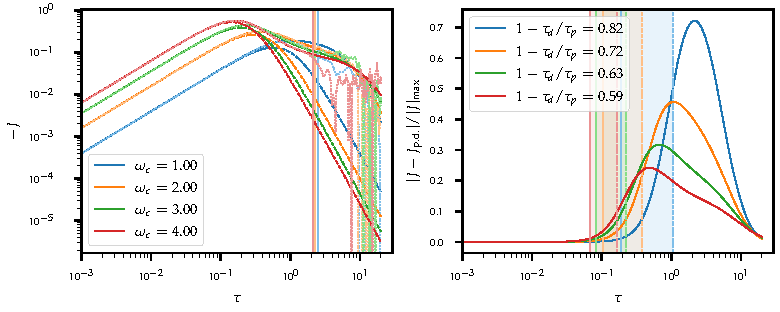
\includegraphics{figs/one_bath_syst/omega_initial_slip}
  \caption{\label{fig:omega_initial_slip} Left panel: The bath energy
    flow of the model \cref{eq:one_qubit_model} for various coupling
    strengths (solid lines) and the pure dephasing flow of
    \cref{sec:pure_deph} (dashed lines). The dotted lines show the
    flow calculated from one trajectory and the vertical lines mark
    the position of the peak of the absolute value of the interaction
    energy. Right panel: The difference of the actual flow \(J\) and
    the pure dephasing flow \(J_\mathrm{p.d.}\). The solid vertical
    lines mark the time \(τ_p\) where the normalized deviation from
    pure dephasing is \(10^{-2}\) and the dashed vertical lines show
    the position of the peak flow at time \(τ_p\).}
\end{figure}

Returning to the simulations in \cref{fig:omega_systematics_system},
we see in \cref{fig:omega_initial_slip} that the pure dephasing
dynamics discussed in \cref{sec:pure_deph} dominate for very short
time scales, but fail to predict the exact location of the peaks. The
deviation from the pure dephasing flow occurs before the peak, where
the time difference between the peak absolute flow and the deviation
increases with decreasing \(ω_c\), as does the magnitude of the
maximal relative deviation. This can be ascertained from the legend of
\cref{fig:omega_initial_slip} where the difference between deviation
and peak time normalized by peak time is given.

For longer bath memories along with weaker
couplings, the role of the system Hamiltonian dynamics in modulating
the flow becomes increasingly important.

Remarkably, the flow for a single trajectory does match the converged
flow even better than the pure dephasing flow. For large \(ω_{c}\) the
single trajectory matches until after the peak, whereas the deviation
occurs earlier for the \(ω_{c}=1\) case. For short times the flow is
mainly influenced by the buildup of the auxiliary states rather than
the fluctuations of the stochastic process, leading to a similar
behavior for most trajectories. See \cref{fig:flow_buildup} an
illustration of this phenomenon. This is useful, as this period of
rapid dynamics must be resolved very precisely to accurately integrate
the flow into the bath energy change.
\begin{figure}[h]
  \centering
  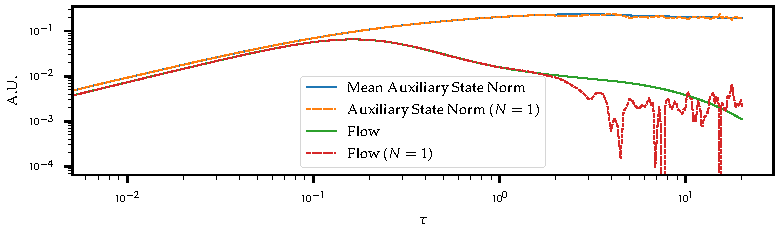
\includegraphics{figs/one_bath_syst/flow_buildup}
  \caption{\label{fig:flow_buildup} The total norm of the first
    auxiliary states and the flow for one trajectory and as a mean
    over all trajectories for the \(ω_{c}=4\) simulation. For short
    times the results for one trajectory match the ensemble means. The
    divergence between one trajectory and the ensemble occurs at
    roughly the same time for the flow and the auxiliary state
    norm. Moreover, flow and mean auxiliary state have the same
    functional form for very short times, apart from a scaling factor.}
\end{figure}

\subsection{Dependence on the Coupling Strength}
\label{sec:one_bathcoup_strength}
After having studied the dependence of the bath energy flow for
various cutoff frequencies of the BCF in \cref{sec:one_bath_cutoff},
we now consider the case with fixed cutoff \(ω_c=2\) but varying
coupling strength. The simulation parameters are the same as in
\cref{sec:one_bath_cutoff} and again consistent results have been
obtained as can be gathered from
\cref{fig:delta_interaction_consistency} throughout the whole range of
coupling strengths.
\begin{figure}[h]
  \centering
  \includegraphics{figs/one_bath_syst/δ_energy_overview}
  \caption{\label{fig:delta_energy_overview} Energy overview for the
    model \cref{eq:one_qubit_model} for various coupling
    strengths. The curves are converged out, and the error funnels are
    not visible.}
\end{figure}

\begin{wrapfigure}[17]{o}{0.3\textwidth}
  \centering
  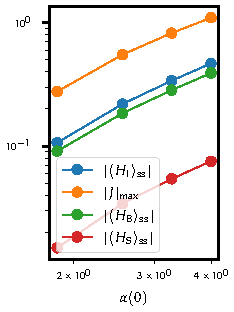
\includegraphics{figs/one_bath_syst/final_states_flows}
  \caption{\label{fig:delta_fs_flow} The absolute difference of the state energies and the
  maximal flows for the simulations in
  \cref{fig:delta_energy_overview} relative to their value at \(α(0)=1.12\).}
\end{wrapfigure}
The interaction strength was chosen linearly spaced and the simulation
results are presented in \cref{fig:delta_energy_overview}.

As the shape of the BCF is not altered the bath energy flows look very
similar as do the interaction energies. The main difference is the
magnitude of the interaction energy. With increased coupling strength
there is an increased interaction energy and an increased flow which
leads to faster energy loss in the system and faster energy gain of
the bath. The stronger the coupling, the more pronounced as the
non-monotonicity in time of the interaction energy, which is reflected
in a non-monotonicity in the bath energy expectation value, which
reaches a maximum and falls slightly for the strongest coupling
simulations. If the interaction is strong enough, ``backflow'' can
occur despite finite bath correlation times. In
\cref{fig:markov_analysis_steady} the bath memory is long,
additionally to a strong coupling so that multiple oscillations can be
seen.

Despite these differences for finite times, the approximate steady
state\footnote{excluding the \(α(0)=0.4\) cases} interaction energies,
maximal flows, system energies and bath energies are almost linearly
dependent on the coupling strength \(α(0)\) as is demonstrated in the
log-log plot \cref{fig:delta_fs_flow}.

We find that we can control the speed of the energy transfer between
bath and system with the coupling strength at the cost of greater
steady state interaction energy. Were we to turn off the interaction
very fast, we would have to expend this energy in the worst
case. Also, both the final system and bath energies are increasing
with the coupling strength, compensating for the interaction energy.
The cooling performance for a coupling that is being turned off at the
end would depend on the concrete protocol as we've seen in
\cref{sec:one_bath_cutoff} and a more detailed study is left to future
work. The interplay between the interaction time-scale mediated by the
coupling strength, the bath memory time and the system dynamics allows
for intricate tuning.


\fixme{iftime: re-run with same coupling strength, more cutoff freqs,
  less samples, see, longer times for coupling strengths, more coup}


\section{Modulation of System and Interaction for a Single Bath}
\label{sec:singlemod}

Because the HOPS allows us to simulate a full dynamical picture of our
model, let us now turn to a situation where the dynamics are of
interest.

A classical dictum of thermodynamics is, that it is impossible to
extract energy from a single bath in a cyclical manner. Indeed, we
found in \cref{sec:ergoonebath} that this also holds for a finite
quantum system coupled to a thermal bath. In \cref{sec:explicitergo}
we found, that the bound given on the ergotropy in such a situation
can be saturated for infinite baths, such as the ones used with
NMQSD/HOPS. However, it is unclear if such a unitary transformation
can be implemented without explicit construction of a model. Our goal
in this section is to extract as much energy from a one-bath system
as is possible without extensive tuning.

In this section we will focus on the minimal dimensionless model
\begin{equation}
  \label{eq:one_qubit_model_driven}
  H = \frac{1}{2} \bqty{(σ_z+1)+λΔ \sin(Δτ) σ_{f}} + \frac{1}{2}
  {\sin[2](\frac{Δ}{2}τ)} ∑_λ\qty(g_λ σ_x^† a_λ + g_λ^\ast
  σ_x a_λ^†) + ∑_λ ω_λ a_λ^\dag a_λ,
\end{equation}
where \(λ,Δ\geq 0\) and \(f\in \{z, y\}\). The form of the system
Hamiltonian has been chosen similar to \cite{Mukherjee2020Jan}, where
Floquet theory was used, and it was shown that the relevant quantities
are scaling with \(λ\). For \(λ=0\) the system Hamiltonian is positive
semi-definite with the energies zero and one.  The modulation of the
interaction has been chosen heuristically to always act in the same
``direction'' and vanish periodically. We choose the ``down state''
with \(H(0)\ket{0}=0\) as initial state, as we want to extract energy
from the bath and not the system. To maximize energy flow, we will use
resonant baths whose spectral densities have been shifted such that
their maxima coincide with \(1 + Δ\).

For this model the ergotropy bound \cref{eq:ergo_bath_change}
evaluates to
\begin{equation}
  \label{eq:ergo_mod_model}
  \mathcal{W} \leq β^{-1} \ln(1+\eu^{-ωβ})=\mathcal{W}_{\mathrm{max}}.
\end{equation}
For \(ω\to ∞\) we find \(\mathcal{W} = 0\) as the temperature \(T\)
must be of the order of the system energy gap \(ω\) for any
energy lowering process to take place.

\subsection{Quantum Friction}
\label{sec:quantum_friction}
Before focusing on the \(λ = 0\) case, we will briefly visit a
phenomenon coined ``Quantum Friction'', whereby the creation of
coherences in the system energy basis hinders the performances of
thermal quantum machines. These coherences raise the ergotropy of the
system without necessarily raising its energy and can thus not
contribute to the operation of a machine.

A simple demonstration of this can be observed in
\cref{fig:quant_frict}. Here the simulation with frictionless
modulation \(σ_{f}=σ_{x}\) does extract less energy from the total
system as \(σ_{f}=σ_{z}\) case. One reason for this is the not
insignificant buildup of ergotropy in the system state which is being
reduced to zero periodically, but does retard the energy extraction so
that less energy is extracted before the periodic steady state is
being reached which does only increase energy (see
\cref{sec:operational_thermo}).\fixme{TODO: plot coherences}
\begin{figure}[h]
  \centering
  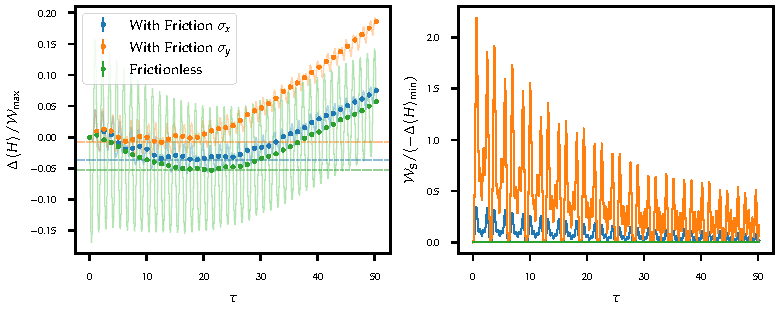
\includegraphics{figs/one_bath_mod/quantum_friction}
  \caption{\label{fig:quant_frict} Total energy change normalized by
    the maximal ergotropy in the left panel and the ergotropy of the system
    state \(ρ_{\sys}\) normalized by the maximal extracted energy
    (dashed lines in left panel) in the right panel over time. Here
    \(λ=0.1, Δ=5, T=5\) was chosen. In the ``With Friction'' case
    \(σ_{f}=σ_{x,y}\) and in the ``Frictionless'' case
    \(σ_{f}=σ_{z}\).  The solid dots mark the times when \(H_{\inter}
    = 0\). The horizontal dashed lines mark the minimal
    total energy differences achieved.  For more parameters see
    \cref{tab:plus_friction}.}
\end{figure}

When choosing \(σ_{f}=σ_{y}\) the situation is even worse, because now
the system modulation does not even commute with the interaction. The
extracted energy is smallest and the relative system ergotropy buildup
is maximal.

\subsection{System Modulation}
\label{sec:sys_mod_v_no_sys_mod}
As it turns out, the modulation generically leads to a deterioration
of energy extraction performance for the model
\cref{eq:one_qubit_model_driven} as is demonstrated in
\cref{fig:quant_frict_sys_no_sys}. Again, the ``friction'' (system
ergotropy) generated by the system modulation is much greater than
without system modulation. However, it is questionable whether this is
the only reason for the performance advantage of the case without
system modulation. Another factor is, that the system goes in and out
of resonance with the bath and therefore hampers energy
extraction.
\begin{figure}[h]
  \centering
  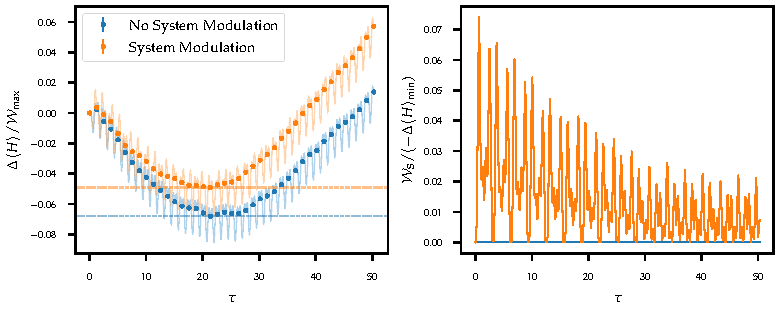
\includegraphics{figs/one_bath_mod/system_vs_no_system}
  \caption{\label{fig:quant_frict_sys_no_sys} Similar to
    \cref{fig:quant_frict}, but for (frictionless) system modulation
    and no system modulation. The parameters were \(λ=0.1, Δ=5, T=5\)
    and further details can be found in \cref{tab:plus_system}.}
\end{figure}

In light of this result we shall continue with \(λ=0\), which
simplifies the situation.

\subsection{Energy Extraction with different Bath Memories}
\label{sec:extr_mem}
To further answer whether a substantial fraction of the maximal
ergotropy can be extracted from a system we have numerically optimized
the coupling strengths of the model \cref{eq:one_qubit_model_driven},
so that over ten modulation periods \(τ_{m} = \frac{2 π}{Δ}\) the
maximal absolute interaction energy is close to a give value (here
\(\ev{H_{\inter}}\approx 0.4\) which constitutes quite a strong
coupling) for various cutoff frequencies \(ω_{c}\).
\begin{figure}[h]
  \centering
  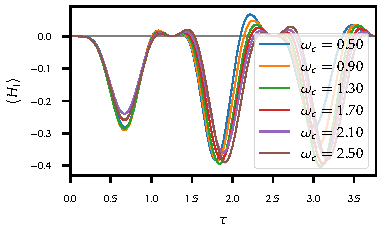
\includegraphics{figs/one_bath_mod/omega_interactions}
  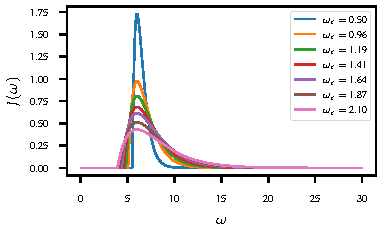
\includegraphics{figs/one_bath_mod/omega_sd}
  \caption{\label{fig:omega_couplings_and_energies} The interaction
    energies and (zero temperature) spectral densities for the
    simulations in this section. Here we used \(λ=0.1, Δ=5, T=5\) and
    the parameters in \cref{tab:plus_omega}.}
\end{figure}

The resulting couplings can be found in
\cref{fig:omega_couplings_and_energies}. They correspond roughly to
demanding \(α_{β}(0)=1.4\), where \(α_{β}\) is the finite temperature
bath correlation function.
\Cref{fig:omega_couplings_and_energies} also shows that for the
simulations with small \(ω_{c}\) the positive parts of the interaction
energy are especially large.

For very weak coupling \(\ev{H_{\inter}}\approx .01\)
\cref{fig:omega_couplings_weak} shows that this optimization procedure
yields the normalization of \cref{eq:normohmic}. This is plausible,
because for weaker coupling the initial slip phase upon which
\cref{eq:normohmic} is based stays valid for longer times\fixme{do
  optimization for more periods / slower mod}, albeit that no
modulation was assumed to derive the normalization. For weak coupling,
only the peak value of the spectral density is important and therefore
the peaks must coincide for similar coupling strength.

In \cref{fig:omegas_total} we see the energy extraction behaviour of
the model for various cutoff frequencies.
\begin{figure}[h]
  \centering
  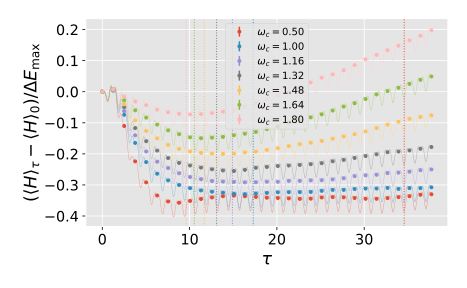
\includegraphics{figs/one_bath_mod/omegas_total}
  \caption{\label{fig:omegas_total} The total energy differences of
    \cref{eq:one_qubit_model_driven} for various \(ω_{c}\). For
    details of the parameters see
    \cref{fig:omega_couplings_and_energies}. The dots mark the times
    when the interaction is turned off.  The dashed lines show the
    position of the where the total energy is minimal.}
\end{figure}
It is clear, that a lower cutoff frequency is advantageous as the
minimal total energy is achieved earlier and is of greater
magnitude. Further, we see that a non-trivial amount of energy is
being extracted relative to ergotropy bound \cref{eq:ergo_mod_model}.

\begin{figure}
  \centering
  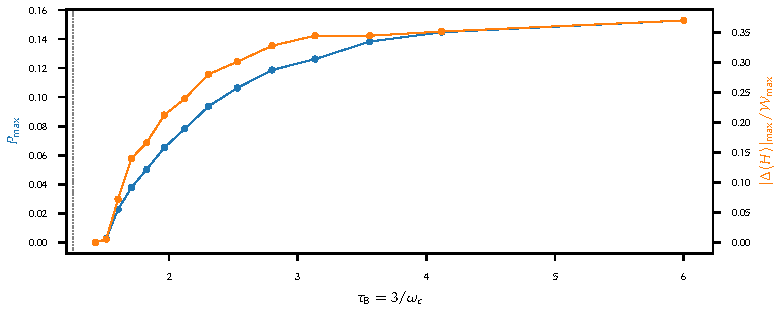
\includegraphics{figs/one_bath_mod/omega_energies_and_powers}
  \caption{\label{fig:omegas_energies_and_powers} One shot power
    (blue) and maximal extracted energy (orange) as a function of
    the bath memory. The grey vertical line marks one
    modulation period.}
\end{figure}
In \cref{fig:omegas_energies_and_powers} we can see that longer
bath\fixme{looks like ``phase transition'' but really isn't} memories,
defined as the time point at which \(α(τ_{\bath}) = α(0)/10\), lead to
both increased energy extraction and increased one shot power. The one
shot power is defined as
\begin{equation}
  \label{eq:one_shot_power}
  P_{\max}=\max_{n\in\NN}\frac{\abs{Δ\ev{H}_{n τ_{m}}}}{n τ_{m}},
\end{equation}
where \(Δ\ev{H}_{τ}= \ev{H}_{τ} - \ev{H}_{0}\).  The concrete shape of
the curve \cref{fig:omegas_energies_and_powers} is hard to discuss
because of the nontrivial shape and magnitude of the spectral
densities. However, the abrupt transition to zero for short memories
is due to the requirement that power and extracted energy have to be
finite, and the stroboscopic time view induced by the requirement that
the interaction energy should be zero.

In conclusion we can say that in the cases studied here we can extract
a finite amount of energy from the system as soon as the bath memory
is somewhat longer than the modulation period. This statement depends
on the definition of the memory time \(τ_{\bath}\) and therefore be
taken as a rule of thumb.

\subsection{Modulation Frequency and Speed Limit}
\label{sec:speedlim}

Another interesting parameter to tune is the modulation frequency
\(Δ\), or equivalently the modulation period time \(τ_{p}=2π/Δ\). In
driven systems, there usually appears a ``quantum speed limit'' that
limits the power output of a driven system at a given coupling
strength. An example is the transition from engine to refrigerator in
a continuously coupled two-bath engine in
\cite{Mukherjee2020Jan}. More generally, this issue is connected to
non-adiabatic changes in the Hamiltonian that can generate non-passive
states \cite{Binder2018}.

Intuitively speaking, slower modulation allows more time for the
system-bath interaction that enables energy extraction from the
initially passive bath state in the first place.

The continuous power is given by
\begin{equation}
  \label{eq:power_for_onequbit}
  P = \ev{\dot{H}_{\inter}} \sim Δ \sin(Δ) \ev{B σ_{x}^{†} + \hc},
\end{equation}
where \(H_{\inter, m} \equiv \ev{B σ_{x}^{†} + \hc}\) constitutes the
unmodulated interaction Hamiltonian. Increasing the frequency \(Δ\)
will increase the amplitude of \cref{eq:power_for_onequbit}. On the
other hand, if the expectation value of \(H_{\inter, m}\) does not
change much, or on a much slower scale than \(τ_{p}\) because of too
fast modulation the \(Δ\sin(Δ)\) factor will cause the expression to
average out to zero (Zeno-like effect, \cite{Kurizki2021Dec}).

Stronger coupling will lead to a greater expectation value of
\(H_{\inter, m}\) and generically to more power.

To assess the behaviour with regard to coupling and modulation speed,
we simulated the model for \(ω_{c}=1\) up to the time \(τ=20\) and
plotted the one shot power \cref{eq:one_shot_power} in a heatmap in
\cref{fig:power_heatmap}. The coupling strength is quantified by the
value of the thermal bath correlation function \(α_{β}\) a time
zero. This balances the shifting of the spectral density for the
different values of \(Δ\).
\begin{figure}[htb]
  \centering
  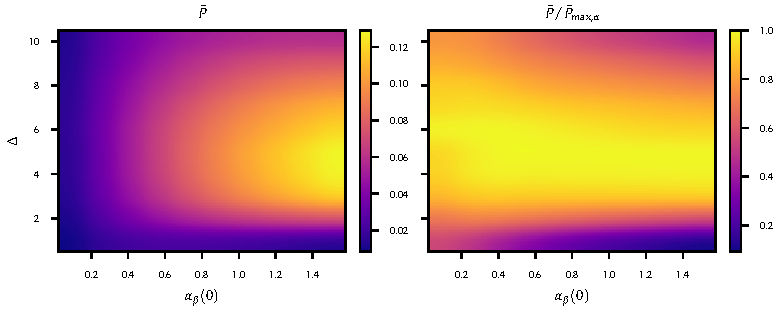
\includegraphics{figs/one_bath_mod/power_heatmap}
  \caption{\label{fig:power_heatmap} Left panel: The one shot power
    \cref{eq:one_shot_power} for the model
    \cref{eq:one_qubit_model_driven} for various modulation
    frequencies \(Δ\) and coupling strengths. The parameters
    \(ω_{c}=1,λ=0.1, T=5\) were used. Right panel: The same, but
    normalized to the maximum power for each \(α_{β}(0)\). In both
    cases \(100\) grid points and Gaussian interpolation have been
    used.}
\end{figure}

We find that the best power output is achieved by stronger
coupling. The dependence on the modulation frequency is more
nuanced. If the power output is normalized by its maximum value for
each \(α_{β}(0)\) it can be seen, that the optimal power output is
achieved at roughly the same modulation frequency. However, with
increasing coupling strength, the system becomes more sensitive to the
modulation frequency, exhibiting a clear maximum. This constitutes the
``speed limit'' discussed above.

\begin{figure}[htb]
  \centering
  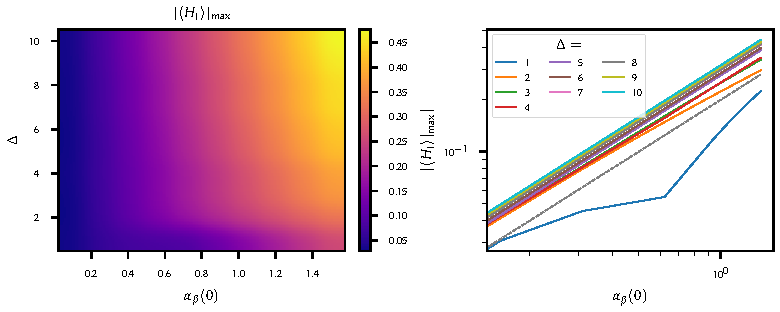
\includegraphics{figs/one_bath_mod/interaction_nontuned}
  \caption{\label{fig:interaction_nontuned} Left panel: Similar to
    \cref{fig:power_heatmap} but showing the maximal absolute
    interaction energies. Right panel: A log-log-plot of the maximal
    interaction energy over the coupling strength. The dashed grey
    line is a linear reference curve.}
\end{figure}

The maximal absolute interaction energies are shown in
\cref{fig:interaction_nontuned} and increase generally with increasing
coupling strength. The dependence on the coupling strength is linear
for modulations with \(Δ\geq 5\) but deviates for slower
modulation. This may be due to the fact, that fewer periods can occur
in the given time frame.

The interaction energy also increases for faster modulation,
especially at greater coupling strengths. Comparing
\cref{fig:interaction_nontuned} with \cref{fig:power_heatmap} we see
that the top right region where the interaction energy is strongest
somewhat coincides with a decrease in power. In this region, the
dependence of the interaction energy on the modulation frequency is
also most pronounced.

Summarizing, we found that the one shot power output for the model
\cref{eq:one_qubit_model_driven} has a complex dependence on the
coupling strength and the modulation frequency. Especially for strong
coupling, the modulation frequency has to be chosen carefully if
maximum energy extraction is desired.

\subsection{Resonance Behaviour of the One Shot Power}
\label{sec:modcoup_reso}

Finally, after having introduced the shift of the spectral density on
a rather vague basis, we would like to give a short example of its
validity.

For this we choose the spectral densities with their peaks slightly
shifted away from \(1+Δ\) to \(1+Δ+δ\) and normalized so that their
peak height is fixed.
\begin{figure}[htb]
  \centering
  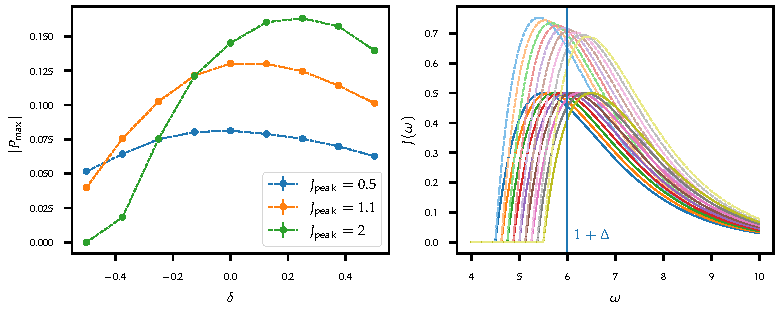
\includegraphics{figs/one_bath_mod/modulation_tuning}
  \caption{\label{fig:modulation_tuning} Left panel: The one shot
    power \cref{eq:one_shot_power} normalized for multiple values of
    the detuning \(δ\) and two peak heights. Right panel: The spectral
    densities for the peak height \(J_{\mathrm{peak}} = 0.5\). The
    dotted lines are the positive frequency parts of the effective
    finite temperature spectral density. The detailed model and
    simulation parameters can be found in \cref{tab:plus_tune}.}
\end{figure}

\Cref{fig:modulation_tuning} shows the result. In all cases, the one
shot power \cref{eq:one_shot_power} as a function of \(δ\) exhibits a
clear maximum which demonstrates the resonance effect.

For the stronger coupling case we find in \cref{fig:modulation_tuning}
that the optimal peak position has moved slightly to the right.
Also the penalty for being off resonant in the negative \(δ\)
direction is much more severe than in the weaker case.

An explanation for the first observation may be, that higher harmonics
like \(1+ 2 Δ\) become important for stronger coupling. Shifting the
spectral density slightly to higher frequencies then optimizes the
coupling.



\section{Quantum Otto Cycle}
\label{sec:otto}

As a demonstration of a standard thermodynamic cycle that is a popular
model in the literature\footnote{See
  \cite{Wiedmann2021Jun,Karimi2016Nov,Binder2018}.}
is a cyclic quantum heat engine that inspired by the Otto
cycle. Similar to expansion and compression of an ideal gas, we
modulate the level spacing of our working medium. This model servers
as a good demonstration of HOPS' capabilities in terms of being a
method that can treat various bath correlation functions and arbitrary
modulations.

Here, we consider a spin boson model much like the one in
\cref{sec:singlemod} but with two baths
\begin{equation}
  \label{eq:otto_model}
  H = \frac{1+f(t)}{2} (σ_z+1) +
   ∑_{i\in\{h, c\}}\bqty{h_{i}(t) ∑_λ\frac{1}{2}\qty(g_{λ,i} σ_x^† a_{λ,i} + g_{λ,i}^\ast
  σ_x a_{λ,i}^†) + ∑_λ ω_{λ,i} a_{λ,i}^\dag a_{λ,i}.}
\end{equation}

The modulations \(f\) and \(h_{i}\) are periodic and constructed out
of smoothstep\footnote{See \cref{sec:smoothstep}.} functions. Rather
than giving the precise formulas, we instead plot all the modulations
over one period in \cref{fig:ottomod}.
\begin{figure}[ht]
  \centering
  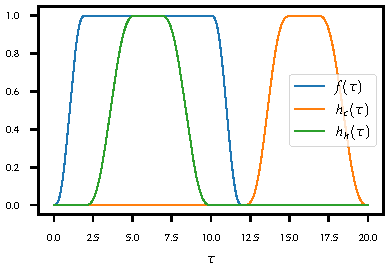
\includegraphics{figs/otto/modulation}
  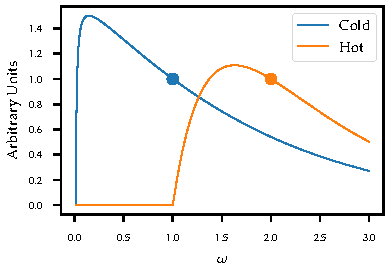
\includegraphics{figs/otto/spectral_densities}
  \caption{\label{fig:ottomod} Left panel: One period of the modulation functions
    in \cref{eq:otto_model}. Right panel: The spectral densities of
    the hot and cold baths. The dots mark the level spacing of the
    system Hamiltonian in the cold and hot phase.}
\end{figure}

First, the energy gap is widened from one to two (widening
stroke). After this, the system is coupled to a hot bath to ``charge''
for some time and decoupled before the energy gap is being compressed
from two to one again (shrinking stroke). Finally, the qubit is being
``reset'' by shedding energy into a low temperature bath.

The effective finite\fixme{explain that?} temperature spectral
densities with \(ω_{c}=1\) have been shifted, such that their value is
maximal for a given temperature at the frequency of the system in its
compressed (cold) or expanded (hot) state. Their magnitudes have been
chosen so that their values at these points are the same as can be
seen in \cref{fig:ottomod}.

We initialize the system in the \(H_{\sys}\ket{0}=0\) state.  For the
demonstration we chose \(T_{c}=1\) and \(T_{h}=20\) so that both
temperatures are finite but not so high that an unreasonable number of
samples is required for convergence. The interaction strength has been
chosen to be relatively weak for the same reason and to be closer to
the known weak coupling realm.

In comparison to the system time scale, the modulation cycle is rather
slow. On the other hand, the time scales on which \(f\) and \(h_{i}\)
change are rather short.

\begin{figure}[ht]
  \centering
  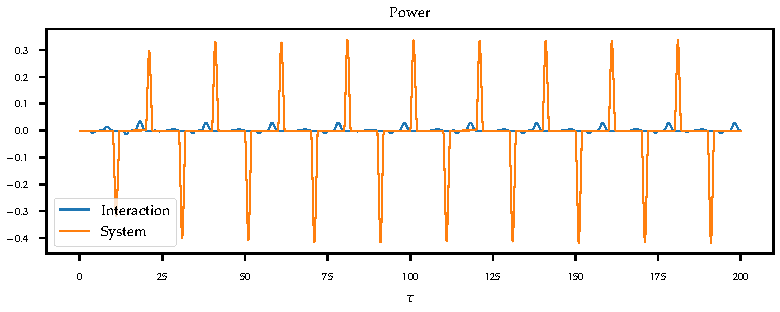
\includegraphics{figs/otto/power}
  \caption{\label{fig:ottopower} The power due to the system and the
    bath modulation of the Otto cycle model \cref{eq:otto_model}. The
    total power is
    \(\ev{\dot{H}} = \ev{\dot{H}_{\sys}} + \ev{\dot{H}_{\inter}}\). }
\end{figure}
\Cref{fig:ottopower} shows the power due to the modulation of the
system and the interaction Hamiltonians. The main contribution to the
power is the system modulation. The shrinking stroke produces negative
(usable) power and the widening produces positive power that has to be
provided externally. More importantly however, we find that also the
modulation of the interaction, i.e. the coupling and decoupling
produce predominantly positive power that has to be put in. In a weak
coupling scheme, this contribution can be neglected. Not so however in
the generic case presented here.

The mean power output of this cycle is
\(\bar{P}=0.002468\pm 0.000021\) with an efficiency of
\(η=29\%\). Neglecting the energy change due to the coupling
modulation we find instead \(\bar{P}=0.004337\pm 0.000018\) and
\(η=52\%\).  This efficiency is, maybe coincidentally, close to the
efficiency given in \cite{Geva1992Feb} for the quantum Otto cycle
under equilibrium conditions. In any case we are far from the Carnot
efficiency for the given temperatures \(η_{c}=95\%\), as we are not in
the adiabatic regime.

\begin{figure}[ht]
  \centering
  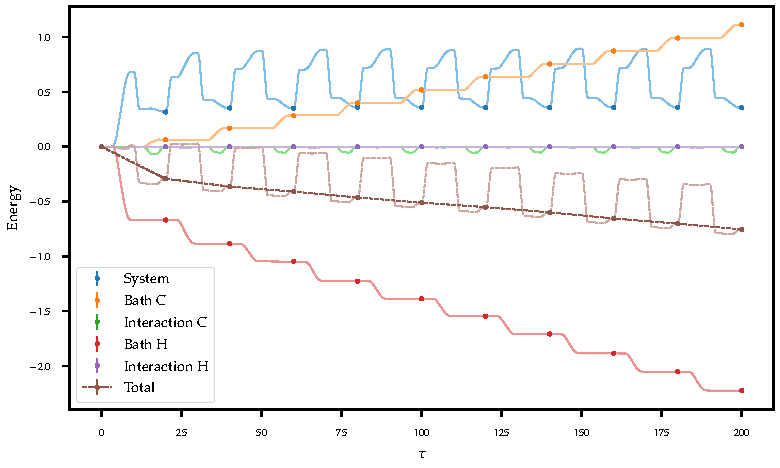
\includegraphics{figs/otto/energy_strobe}
  \caption{\label{fig:ottoenergy} The system, bath and interaction
    energies as well as the total energies of the model
    \cref{eq:otto_model}. The dots mark the times where one cycle is
    completed.}
\end{figure}

In \cref{fig:ottoenergy} we show the full energy dynamics. The
interaction energy for the coupling to the hot bath is almost
negligible, while the interaction with the cold bath is stronger. The
system energy change due to the both is of similar magnitude however.
A periodic steady state is reached after roughly two cycles. In this
steady state, the system and interaction related quantities are
constant in the stroboscopic view (the dots in \cref{fig:ottoenergy}),
while the total energy and the bath energies depend linearly on
time. We do not see no oscillations in the bath energy which would
indicate the more complicated energy transfer behaviour we found in
\cref{sec:one_bath_cutoff}, signifying that we are working in a rather
``tame'' regime as intended.

The Gibbs like inequality \cref{eq:secondlaw_cyclic} derived in
\cref{sec:operational_thermo} can also be verified in this case.
We find
\begin{equation}
  \label{eq:secondlaw_otto_actual}
  ∑_iβ_i ΔE_{\bath^i}^\cyc = 0.1096\pm 0.0008 ≥ 0,
\end{equation}
which does satisfy the inequality to over 100 standard
deviations. Minimizing this quantity would maximize the efficiency.

A worthwhile task for future work would be to verify the results
summarized in \cite{Binder2018} for the Otto cycle. Especially the
optimization for optimal power which leads to the
Novikov–Curzon–Ahlborn efficiency \(η_{ca}=1-\sqrt{T_{c}/T_{h}}\) is
interesting in the case of stronger coupling.

With this cycle, little coherence is generated\footnote{See
  \cref{eq:otto_coherences}.} leading so called ``frictionless''
dynamics. See also \cref{eq:otto_bloch} for a plot of the trajectory
of the system density matrix in the bloch sphere.


Another interesting cycle to study would be a Carnot-type cycle, where
the modulation of the system and the thermalization with the bath
occur at the same time. Interpolating between Otto and Carnot, as well
as studying the effect of overlapping and shifting strokes is a
fascinating avenue for exploration.

Also more interesting working media, such as a three level system are
of interest. In \cite{Uzdin2015Sep} it is shown, that in certain
regimes quantum coherence can lead to superior power output. In the
same regime different types heat engines are equivalent. Both these
effects have been observed experimentally in \cite{Klatzow2019Mar}. It
would be interesting to see if the slight deviations from theory in
\cite{Klatzow2019Mar} could be explained using HOPS.


\newpage
\section{Anti Zeno Engine}
\label{sec:antizeno}


\section{Miscellaneous Demonstrations of the Capabilities of HOPS}
\label{sec:miscdemo}
Very short mention of some results from ``side projects'' if I have
the time to include them.

\begin{itemize}
\item two qubits coupled to each other -> steady state flow
\item otto cycle
\item rotating engine
\end{itemize}

\section{Some Proposals for future Work}
\begin{itemize}
\item ... list all those nice papers ...
\item the third law
\item look more deeply into the peculiarities in \cref{sec:oneosccomp}
\item verify speculation of energy flow vs non-markvianity: flow
  between two baths though a system
\item three level system -> paper
\item driven spin boson -> paper \cite{Magazzu2018Apr}
\item flows crossing in one point: robust featureu
\item linear regeime of steady state energies -> universal, how far
  does it extend
\item more detailed parameter scans, universality between different models?
\item state changes -> is energy difference = heat + work path
  independent (maybe try different protocols and turn off interaction
  at for beginning and end in an adiabatic way...)
\item compare with results from master equation in \cref{sec:prec_sim}
\item steady state methods, better convergence for long-time
  simulations
\item coupling to single bath: although breach of second law forbidden
  -> cyclical energy transfer for very long bath correlation times
\item filter mode: \cref{sec:shift_sp}
\item otto cycle: sensitivity to timing stronger with stronger coupling?
\end{itemize}
